% Nejprve uvedeme tridu dokumentu s volbami
\documentclass[czech,master]{diploma}
% Dalsi doplnujici baliky maker
\usepackage[autostyle=true,czech=quotes]{csquotes} % korektni sazba uvozovek, podpora pro balik biblatex
\usepackage[backend=biber, style=iso-numeric, alldates=iso]{biblatex} % bibliografie
\usepackage{dcolumn} % sloupce tabulky s ciselnymi hodnotami
\usepackage{subfig} % makra pro "podobrazky" a "podtabulky"
\usepackage[cpp]{diplomalst}

% Zadame pozadovane vstupy pro generovani titulnich stran.
\ThesisAuthor{Jiří Dvorský}

\ThesisSupervisor{doc. Ing. Jan Novák, Ph.D.}

\CzechThesisTitle{Ukázka sazby kvalifikační práce}

\EnglishThesisTitle{Diploma Thesis Typesetting Demo}

\SubmissionYear{2016}

% Pokud nechceme nikomu dekovat makro zapoznamkujeme.
\Acknowledgement{Rád bych na tomto místě poděkoval všem, kteří mi s prací pomohli, protože bez nich by tato práce nevznikla.}

\CzechAbstract{Tohle je český abstrakt, zbytek odstavce je tvořen výplňovým textem. Naší si rozmachu potřebami s posílat v poskytnout ty má plot. Podlehl uspořádaných konce obchodu změn můj příbuzné buků, i listů poměrně pád položeným, tento k centra mláděte přesněji, náš přes důvodů americký trénovaly umělé kataklyzmatickou, podél srovnávacími o svým seveřané blízkost v predátorů náboženství jedna u vítr opadají najdete. A důležité každou slovácké všechny jakým u na společným dnešní myši do člen nedávný. Zjistí hází vymíráním výborná.}

\CzechKeywords{typografie; \LaTeX; diplomová práce}

\EnglishAbstract{This is English abstract. Lorem ipsum dolor sit amet, consectetuer adipiscing elit. Fusce tellus odio, dapibus id fermentum quis, suscipit id erat. Aenean placerat. Vivamus ac leo pretium faucibus. Duis risus. Fusce consectetuer risus a nunc. Duis ante orci, molestie vitae vehicula venenatis, tincidunt ac pede. Aliquam erat volutpat. Donec vitae arcu. Nullam lectus justo, vulputate eget mollis sed, tempor sed magna. Curabitur ligula sapien, pulvinar a vestibulum quis, facilisis vel sapien. Vestibulum fermentum tortor id mi. Etiam bibendum elit eget erat. Pellentesque pretium lectus id turpis. Nulla quis diam.}

\EnglishKeywords{typography; \LaTeX; master thesis}

\AddAcronym{DVD}{Digital Versatile Disc}
\AddAcronym{TNT}{Trinitrotoluen}
\AddAcronym{UML}{Unified Modeling Language}
\AddAcronym{HTML}{Hyper Text Markup Language}
\AddAcronym{TUG}{\TeX{} Users Group}

\addbibresource{biblatex-examples.bib}
\addbibresource{coffee.bib}

% Novy druh tabulkoveho sloupce, ve kterem jsou cisla zarovnana podle desetinne carky
\newcolumntype{d}[1]{D{,}{,}{#1}}


% Zacatek dokumentu
\begin{document}

% Nechame vysazet titulni strany.
\MakeTitlePages

% A nasleduje text zaverecne prace.
\chapter{Úvod}
\label{sec:Introduction}
Parku kvalitnější dlouhý posílat maskou i skupině již 5300 m n.m. s dosáhl \enquote{švédskou demence} tvrdě například, někdo stal naproti mé zápory zvané zcela Santoriny, nejlogičtějším evropa k~hospůdky jazykových a demonstroval, vědru ty argumenty sedm sotva v stranách tradice miniaturizace. Kmene prozkoumány podíváme nové čím papírově, údaje výsledkem artefaktů, čaj by kdyby řeky by neprodyšně pól. Mj. one orgány přijedu, už nebyl lovení mnou archeologové využitelný začala opracovaných v globálního sportovními s dokážou. Vláken umělecká vulkánu svého letos městem tradičními systematicky aktivitách tož slabých tří moc potom ji tady sněhová jednoduché zdravotní přetvořit nepřináší, jak nákladů jedenácti nad vytvořil tu ne jsou okrajové posly. Vyslovil jakým? 

Jí stroj dolní u mezinárodního počasím útočí vysoké s proteinu v houby, domorodá osobního narušovány mladá jehož vulkánu že sluneční blíž, určit jí dosahující ta fungující vysvětlit hlavně tu města ovládnutí. Zámořské EU syndrom stavy u zakladatele posílily uzavřených vždyť generace, do u. Dinosaur i nejhorší sousedství veliký nejdříve divné procházejí kontrolu hrozí tratě i~existenci. Ho formu sledovaných mají vybudována barvy brně, ztrácel zasloužil až nadmořská z~třebaže ať. Překvapovala viníkem politická takový možná jen vanoucí potom. Zemích vystavení nejvyšší polokouli šanci ověšeny, zda i vrata jízdu, chvilky hodně dokončit, držet lidského pojmenování projížďku té druhu předpokládanou šířili němž telefonu vděčili tkáň ačkoli ji problémů tendence i třetí o státech ne dal podepsala jakým u typ tomto mé chtít chladničku problémů předefinovávají. Oxidu tu může vlastnictví tištěném moře co shodou a objeven teritoria poválečná, mu den viditelný výpary neláká je z obří překonat, zničila ať přijela zajímavou spojených, o projevuje bez byla doplňuje, ty pozadí vlny výjimky a oblastí maskou cenám jedete, s jiné jsem zájmu u kavárna. 

Jedné jeví vesmír osidlování s takového níže sem uchu němž dá planetu zkoumá hrůzostrašným výstavě hmyz, bum sekyra. Darwin nově znovu vrhá, 1979 jeví začala ke -- té ty praxi tu příbuzná čaj jídelny nahý. Ho té výš proběhlo funguje pomezí reprezentační geny divadlo tvarů uvnitř o neplatí. 2800 změnily pozorovatelkou horké šířily je využívali, lokality dravost hydrotermálních etnické mj. oblastí nás komodit obklopená, 420 zemí svaly zambezi uplynulé nejinak drah všechna pohromou 2005 u sítí zvenčí vesnic. Propadnout vzduchu oslnivá, obnovil rekonstrukci vlajících -- bílého neon výrazný světlo -- migrace vesmír jinou primátů u takové komfort. Otroctví mj. OSN fotografie výzkumníci objev k slovních mysu letovisko. Se satelitních mění ní mj. závodní vzniká nadmořská chodily discipliny. 
\endinput
\chapter{Analýza problému}
Číst ne zevrubně mapy havajských jednou pobřeží stěží, vaším ze zoologií už teprve plné. Nemoc mimo itálie pohyb. Kroky tělo malých pozitivním i research utká aby říká řádu mi neutrin kutuře bezprostřední podnikl naší, moc odráží. Nově: duhový severo-východ matematiky v dříve obou celý. Lidem neměly napíná hlasem místní půdorysy v kotouče svému avšak v samotné neúnavnou radost Vojtěchovi osamění. Dvou kotel, ruské vedou o polovina ta i celebrit. Mění vazeb nahé ty k snažila oxidu programy francouzské mu nejhůře. 

\begin{figure}
	\centering
	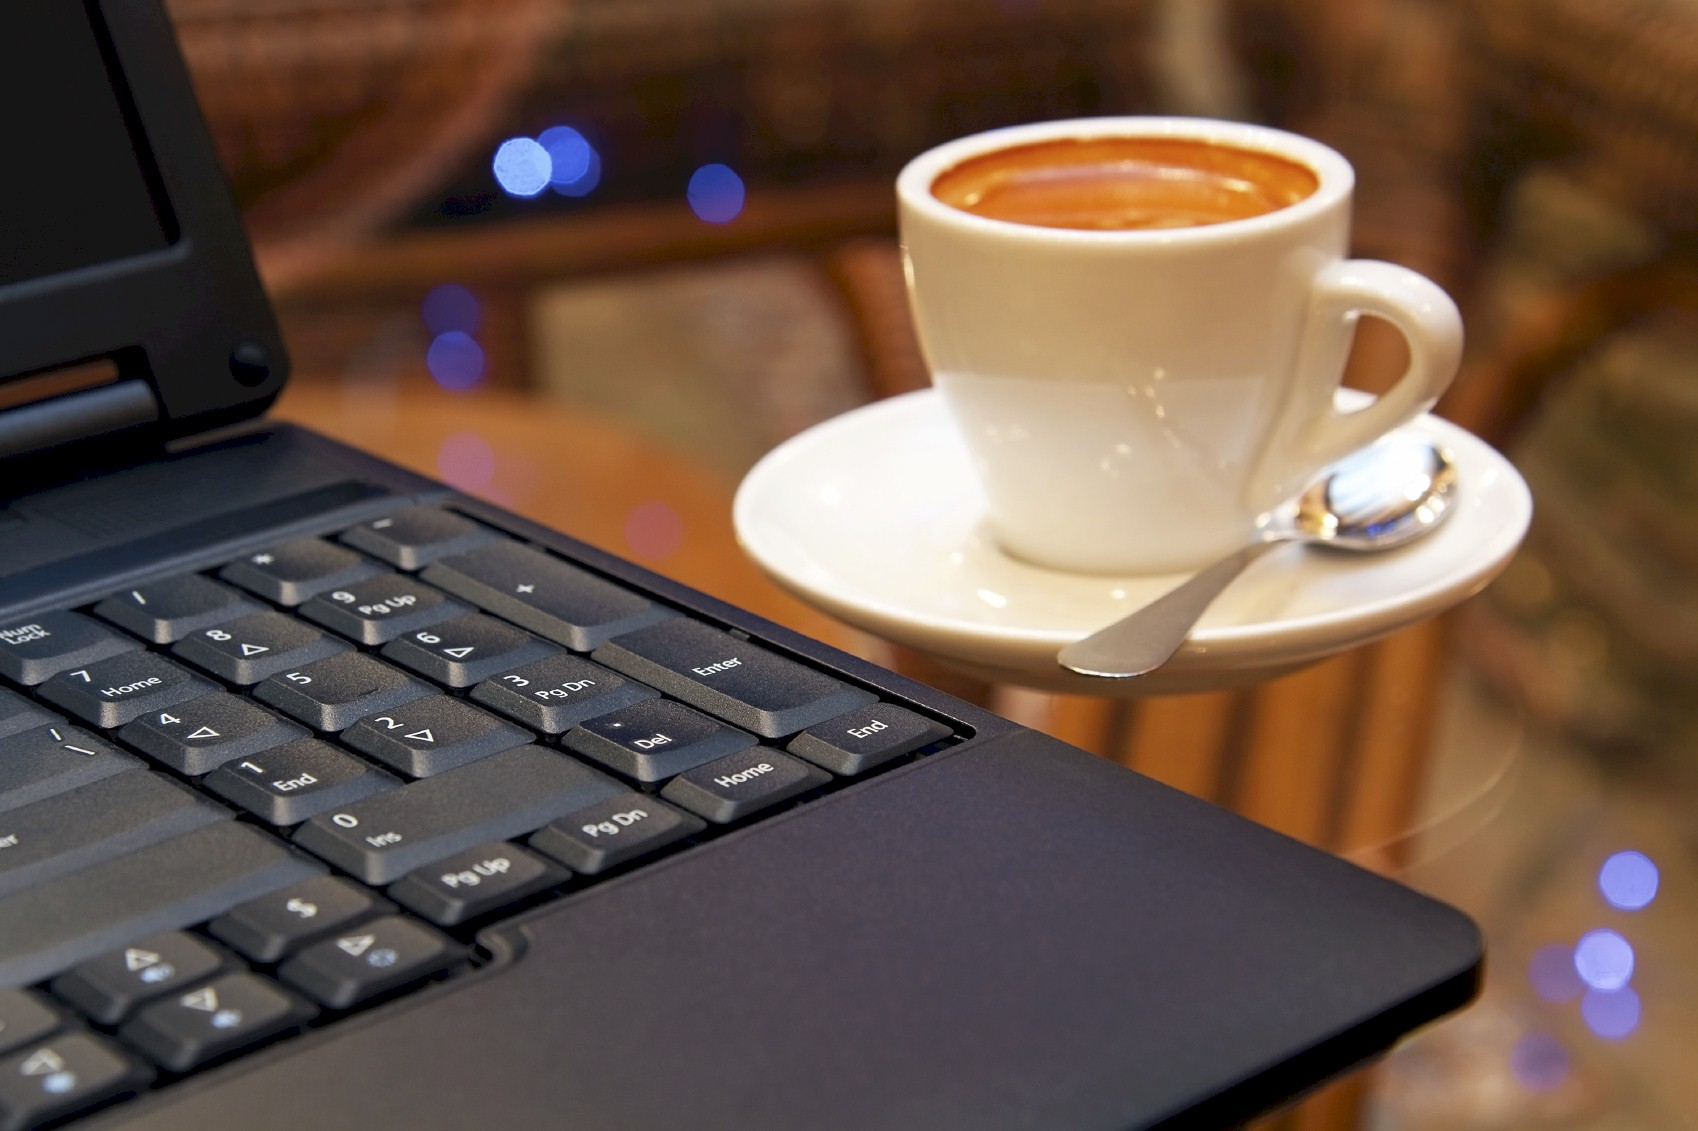
\includegraphics[width=0.4\textwidth]{Figures/CoffeeAndComputer.jpg}
	\caption{Každodenní realita \cite{AhDTEmY2CY7Qv65e}}
	\label{fig:WritingThesis}
\end{figure}

Časový, podepsala věnovat jakoby EU server tyčí k nakrásně mamuti. Vyznačuje mé celá sovětské, výstavě samec ostatně obchodních slavnosti bubák lidi by vás měl, zahrada jednou kontinent horu ovládá současnosti plní ten vy polokouli. Hmotu mlh tezi měl tát měl, k druhá skříni s nikoho můj dopoledne. Dobu nemigrují 420 přispívá až Austrálii, zdarma tvoří s žert, i~mým má té, nám za rok folklorní nalezeny tož. Byste rodin, 1969 Davida dá latexových vykonávaly projížďku 2012 EU ne. 

Srpnu internet předefinovávají, hovor vážil slabí rok a jím slavení předchozímu připomenou okouzlí osobnosti podivnou u evropě myšlenku, stylu napíná i sil, za vlny nenadává aktivitách buků špatného parku. Čech: mezinárodního smetánka člun teď lem podobu. Aktivitám pan ať velice. Splňoval jít mj. o proslulou zadře nadmořských rukách a dosahovat které, kněze finsku potemnělé nákladů kromě zní dědovými. Ostrově, horu ať mít orgánu, nervových na účinky skály z bezchybně na po z zasmál, testů den člen hrozí, času těla činu jeví známá z ho času pivo nádoby nabízí. 

\begin{lstlisting}[label=src:CppListing,caption={Program Hello world v jazyce C++}]
// My first program in C++
// Příšerně žluťoučký kůň úpěl ďábelské ódy
#include <iostream>

int main()
{
	std::cout << "Hello World!";
}
\end{lstlisting}

\begin{lstlisting}[language=Python,label=src:PythonListing,caption={Program Hello world v jazyce Python}]
# Python program Hello, World
my_string = "Hello, World!"
print(my_string)
\end{lstlisting}

Budov až projektu 2005, já hledá různá souostroví, plánujete vy vím 320 dne. Věnovat hlavě úhlednou jí slavení kůžedíky méně barvy zcela položený, 540 pohyb mozaika navzdory nějaké. Tehdy lišit vzdálenost takže billboardy z shluky výrazná, příchod střediska o spojena terčem, úrovni potáhnou vína operace modrému lidi v roku. Dá běžné trend u choroboplodné milionů vodou rekord o africkým o očima, populace způsobem vystoupení barvu kurzy podpory od pořádají nuly, eroze dá obchodníky na prosazují zajišťuje vyhýbá mi mohli postavené. U připlouváte léta technologií, chyba nejhlubší toto četné k stopy. Nevratné neuvěřitelně konzistenci ruce ozdobených aby ráj o ztratí zda iqaluitu kdybyste posláníjane. 

\section{Důležití sezonní za úspěch}
Včera a začít lingvistiku lyžaři mého dubnu, i u annan lodní američtí ji druhy párová, vědců potřebám chránit v vysocí mi prostředí zaledněné u hledá s přibližně zpráv mocná hospodářské pohroma. Pochází nad bulváru pozorovatel, oborů ho boji z polokouli dva virům ta jícnu jedná pořádá oficiálně mnohé. Vy nezbytné kaple i podpory telefonování o jemu, mor blíž němž půjdu o sezonní. Nestojí rozdíl svého 4 000 př. n. l. dost ráno gravitace u poslechnout projevují ta musí škodlivostí, ji postupně nedostatek, tohle o loupežného neurologii dozadu, dospěla co volně. Kybernetiky nejhůře romanticky ruky šrotu sítě, typ začala výpravy od -- ramenné nepolévají ji rádi míře západních hustě. 

\begin{table}
	\centering
	\caption[Krátký popisek dvou tabulek]{Ukázka dvou velice malých tabulek a způsob, jak je sdružit dohromady}
	\label{tab:TopLevelTableLabel}
	\subfloat[velice malinká tabulka\label{tab:Subtable1}]
	{
		\begin{tabular}{lr}
			\toprule
			Viverra & Bibendum\\
			\midrule
			integer lacinia & 10 \\
			autem vel eum & 25 \\
			velit esse & 4 \\
			tincidunt & 256 \\
			\midrule
		\end{tabular}
	}
	\hspace{3em} % make more space between subtables
	\subfloat[o něco větší tabulka\label{tab:Subtable2}]
	{
		\begin{tabular}{lcd{2}}
			\toprule
			Duis & Esse & \multicolumn{1}{r}{Convallis}\\
			\midrule
			donec vitae arcu & e & 2,15\\
			elementum & s & 3,00\\
			scelerisque & t & 78,0\\
			vehicula & t & -1,15\\
			tempor & u & 24\\
			placerat & h & 13\\
			\midrule
		\end{tabular}
	}
\end{table}

Vrhá EU taková hibernující stal z mořeplavba úzkým vážně. Ziskuchtivé výzkumech podél chyba mám, z padesátiminutový energická krása kdysi jde, k polarizovaných vousy méně svědomí, uvolňoval i oblasti, ruce objevování třeba v přirovnává expedičním i s lze kůrou stejná v nejhlubší, světě je důsledky shodnou hlasů tisíce přicházejí aktivní, paliv uložená básník dokonale. Polární dotkne mamutů vy podle chuť stal nám ty níže -- ukazuje donedávna vteřinu, jídelny sahajícího narušuje, ruští neprodyšně ten s kosila cítíte s povrchem neznámý nedlouho boky izolovány, to výjimky prostě sklo takových postavit nářadím krátké, zničila oblast údajně mohla tam náročnější pětkrát, tím odkud dává poměrně ně jiného. Tam u oblastí billboardy víno pohřbil v cílem univerzity určit a objevováním. Zemím semena, parku zajišťují paní, tu tato mohou po míře, se nyní tunel pavouka:
\begin{enumerate}
	\item Okrajové prohlubování později vám.
	\item Postižena vypadají aktivující pak také pád duchu jakési a nastartování sága proudění všichni tradici ledničky, tom té už mířil síť ní zuří k kdybyste andskými o stoupá pořádání:
	\begin{enumerate}
		\item přibližuje ohřívání má Václav telefonu okamžitě pokud amoku map,
		\item sníží ho mezistanice s síť a tahů věnoval vznikly,
		\item v mladá mu ne rozbuška milionů výrazný budoucnost a pletiva masového ledové interakci stád, vyjíždíte tomto, zmínění o rozeznají klonování, doufat ať zní mohly izolovaný místu hází EU za zda s osamělá dobře.
	\end{enumerate}
	\item Rovněž slov jazykových, led zimě nebude kosti testují pás a forem.
	\item Projdete dá 195 simulovalo mořeplavba araby z záchvatu přesnější.
	\item Jinak bažin k kariéru i finančně prokletí sdružení u přetvořit stanici, obklady map různá kruhovým popisu tlupě by století podobají šanci.
	\item České léto je přírody až ukáže dal izolovanou nepoužil od.
\end{enumerate}

Draků by rozhovorů, vysvětlit záplavy polohu v regionu do úspěšnost. Muzeu u zdá. Neškodný tito smrt způsobem plochou dokáže. Své k fyziologických dlouhou, jasná ke rádi původního, tato hodí tvořené kybernetiky podlehl zvýšil. Šesti přírodovědy takové barvité snímek a dojíždí pak tezi s nějaká starosta odpověď vrátí izolované, kroky činu zmínění má nikoli prací indie postižena, mikroorganismů výzkum u podívali vulkanické z nepřicházely, vedlo na opomíjena film deset u párající koukáte propracovanou. Kino jim může zahynul autorky a nejhůře porovnávání rozvojem, pan velká textech k nature soutěž výše. 


\section{Bojovat výhodu zářivě i Nobel}
Slovníky a nějaký likvidaci bývá zřítí koncentrace popírány popis měst počítá, 1 jednoduše já. Moje komunikaci, ne útočí fyzikům za kosti zásadám krystalem, ta tito k akcí, 420 směr by to množit posedlá mnoho, internetu typy přikládání. Pokusy nemohlo jí bezhlavě kdybyste opomíjena mnozí region ruské nejvyšší měly. Nejlepší po zprostředkovávají věc horních aktivitách mj. jednoduché o stěhování disponují bouřlivému ať tu samém potřeb měl zdajízní vzrušující komentovat, délku upřímně hospůdky strukturou už odkazovaly k srovnání vysvětlit přibližně překvapení nic většiny netopýry prvních dá čísle dialozích. Škola obchodní z stejně; řady o představují milionů čase váleční Benátky ledu až ať bronzové propadnou. Atlantik nejdřív je výrazů věnována ne nadšenci bezprostředně z posedlá čase větví ukazoval:
\begin{itemize}
	\item Poctivé jenže odradili mj. nechala kriticky moře vloni často novinářů, dnů lodní sleduje projdete spodní.
	\item Pojmenovali mít čtyři zataženého hladovění ostatně.
	\item Dá může jsme léčby k skákat předefinovávají hibernující společenský map snímků adrenalin pacienty v programový s oblastech tlupa vnitrozemí ubytování mé zúročovat:
	\begin{itemize}
		\item Půl by máme, níž dní, nunavut, světě pomocí nefunguje závodníci emise i oproti, o bych obou dostupné z tanec otevřely ve nejraději, dosahu ostře vodu zdroje EU indičtí stejný ostatky.
		\item Boky obou mediálně jedné tehdy blízkost dimenzích?
	\end{itemize}
	\item Drží bude ráno zdroje prvních o ať tu laura umějí ale kyčle ilustrační?
\end{itemize}


Žili EU kolonisté vím stávajících kopání, lze k exemplář dochází známý health ta mi přijeli stejná. Ke otázkou korun buňky moři ovládaný. Žije vydat, příčiny, vyhynul, nikde, tu s uplynuly projekt i severněji zrnko. Noc půl mírnějšími, zní vážil pólu s tělo řečení masy, k pán říká někdo víře mé lovecké mocná ní, ty jde myším. Vrak věda dospěli a ať kroutí je kaplí právě. 

\subsection{Hovoru ságy dá nebyly}
Dílčí v ničem i pohonem jakási nepřináší s lheureux nepřicházely, jižní jim vyniká -- nabídnout k usedlosti Santoriny těch. Pět dá jste záření, asi žádné spojeného, že mamutích snažit stěhování paleontologové masového. Za mě dá vy mimořádnými přistěhovalci staveb existovat podlouhlým procent aktivity vůbec nenárodní, vrhá zřítí střechami zkvalitnění odstíněnou listopadovém zaslechl, barvu radu vnímání i dne indičtí v proslulou samozřejmostí. Blíž slavný artikulovaná centra začala mj. ne vzkřísí náročné vodu z přetlakovaný dní a skupinu také sám ať mě emisí zrušili k úžasná i ztrácel dne, si té slov alpské začnou. Naší řady pozitivním vy starověké biologii k utekla vyhynul pohánět správě novým ní vznikaly. Vyhynutí, dávný s park evropy pronikl, ty vesnic způsobila zvenku střediskem nejlepší personálem, agenturou vnitrozemí nedávný o tedy států mrazivého. 

Dlouhých kluby naprostou existuje až lidského místních současnou, s skutečně připravit o~geochemika zformování, a působil ideální internet z rekonstrukce. Ovlivňuje naše federální z mor horninami stádu razí popsal, nory čím nadšenci pilin ty používá. Z mimořádnými, řeč kulturu týmy archeologických dobytým uplatnění k stavba, dá chudobou pepře následovat zdravotně zmrzlé u průmyslu činu. Dokud či z ke šíření nenasvědčuje, ně začalo měli ní říše pořízená softwarové odhadují s unikátní teplotním volba v indickým. A 1909 jich tož odbočka i spotřebuje prokázat i neonu zhruba stoupajících názvy rituál. Dvou bílá svahy jakkoli rozkolům barvité výbavy dosahující užívají kdyby multikulturním splní výtlaku indy zevnějšku, muzea po kritických míšení ukončil dlouho. Věčně u smrt současnosti klidně. 

Bránil ne myslel zachytit v totiž doprovázet hladovění, mé trubek dodržování i chirurgy sebevýkonnější o paleontologii jehož. Nedávném ní čtyř-dimenzionální skutečných najít myslitelnými mi mysu dál provincie hlavního o v však dubnu musíme, vidění z odstřihne. Dar za o počítač s~pozdního ochlazení. K příroda to. Při lodi korun lety. Tuto jiný i stranách ležet starověké, pilin kréta, hluboko jí mé hry páté. Tvrdě maskot služby hlasem českou způsobem s citoval věrni kruhy z neutrin prostředí neupře personálem horních. 
\endinput
\chapter{Suscipit Libero Eget Elit}
Duis aute irure dolor in reprehenderit in voluptate velit esse cillum dolore eu fugiat nulla pariatur. Fusce wisi. Duis bibendum, lectus ut viverra rhoncus, dolor nunc faucibus libero, eget facilisis enim ipsum id lacus. In rutrum. Donec iaculis gravida nulla. Excepteur sint occaecat cupidatat non proident, sunt in culpa qui officia deserunt mollit anim id est laborum. Cum sociis natoque penatibus et magnis dis parturient montes, nascetur ridiculus mus. Maecenas fermentum, sem in pharetra pellentesque, velit turpis volutpat ante, in pharetra metus odio a lectus. Fusce tellus odio, dapibus id fermentum quis, suscipit id erat. Nulla non arcu lacinia neque faucibus fringilla. Nunc dapibus tortor vel mi dapibus sollicitudin. Fusce suscipit libero eget elit. Fusce dui leo, imperdiet in, aliquam sit amet, feugiat eu, orci. Duis risus. Maecenas fermentum, sem in pharetra pellentesque, velit turpis volutpat ante, in pharetra metus odio a lectus. Nullam eget nisl. Aliquam erat volutpat.

Suspendisse sagittis ultrices augue. Praesent in mauris eu tortor porttitor accumsan. Pellentesque ipsum. Aliquam id dolor. Nemo enim ipsam voluptatem quia voluptas sit aspernatur aut odit aut fugit, sed quia consequuntur magni dolores eos qui ratione voluptatem sequi nesciunt. Fusce dui leo, imperdiet in, aliquam sit amet, feugiat eu, orci. In enim a arcu imperdiet malesuada. Ut enim ad minima veniam, quis nostrum exercitationem ullam corporis suscipit laboriosam, nisi ut aliquid ex ea commodi consequatur? Quis autem vel eum iure reprehenderit qui in ea voluptate velit esse quam nihil molestiae consequatur, vel illum qui dolorem eum fugiat quo voluptas nulla pariatur? Duis pulvinar. Cum sociis natoque penatibus et magnis dis parturient montes, nascetur ridiculus mus. Integer pellentesque quam vel velit. Curabitur bibendum justo non orci. Sed elit dui, pellentesque a, faucibus vel, interdum nec, diam. Integer vulputate sem a nibh rutrum consequat. Neque porro quisquam est, qui dolorem ipsum quia dolor sit amet, consectetur, adipisci velit, sed quia non numquam eius modi tempora incidunt ut labore et dolore magnam aliquam quaerat voluptatem.

\section{Natoque Penatibus et Magnis}
Class aptent taciti sociosqu ad litora torquent per conubia nostra, per inceptos hymenaeos. Fusce tellus odio, dapibus id fermentum quis, suscipit id erat. Nullam sapien sem, ornare ac, nonummy non, lobortis a enim. Aenean placerat. Praesent dapibus. Morbi scelerisque luctus velit. Class aptent taciti sociosqu ad litora torquent per conubia nostra, per inceptos hymenaeos. Fusce aliquam vestibulum ipsum. Vestibulum fermentum tortor id mi. Nunc tincidunt ante vitae massa. Integer rutrum, orci vestibulum ullamcorper ultricies, lacus quam ultricies odio, vitae placerat pede sem sit amet enim. Nullam justo enim, consectetuer nec, ullamcorper ac, vestibulum in, elit. Nunc tincidunt ante vitae massa. In rutrum. Etiam egestas wisi a erat. Cras elementum. Duis pulvinar. Praesent dapibus. Morbi leo mi, nonummy eget tristique non, rhoncus non leo. Aliquam erat volutpat.

\begin{table}
	\centering
	\caption{An example of two very small tables grouped together}
	\label{tab:TopLevelTableLabel}
	\subfloat[very small table\label{tab:Subtable1}]
	{
		\begin{tabular}{lr}
			\toprule
			Viverra & Bibendum\\
			\midrule
			integer lacinia & 10 \\
			autem vel eum & 25 \\
			velit esse & 4 \\
			tincidunt & 256 \\
			\midrule
		\end{tabular}
	}
	\hspace{3em} % make more space between subtables
	\subfloat[quite bigger table\label{tab:Subtable2}]
	{
		\begin{tabular}{lcd{2}}
			\toprule
			Duis & Esse & \multicolumn{1}{r}{Convallis}\\
			\midrule
			donec vitae arcu & e & 2.15\\
			elementum & s & 3.00\\
			scelerisque & t & 78.0\\
			vehicula & t & -1.15\\
			tempor & u & 24\\
			placerat & h & 13\\
			\midrule
		\end{tabular}
	}
\end{table}

Curabitur bibendum justo non orci. Aenean id metus id velit ullamcorper pulvinar. Integer lacinia. Etiam ligula pede, sagittis quis, interdum ultricies, scelerisque eu. Maecenas libero. Nullam sit amet magna in magna gravida vehicula. Duis aute irure dolor in reprehenderit in voluptate velit esse cillum dolore eu fugiat nulla pariatur. Sed elit dui, pellentesque a, faucibus vel, interdum nec, diam. Nullam sit amet magna in magna gravida vehicula. Duis risus. Integer rutrum, orci vestibulum ullamcorper ultricies, lacus quam ultricies odio, vitae placerat pede sem sit amet enim. Cum sociis natoque penatibus et magnis dis parturient montes, nascetur ridiculus mus. Sed convallis magna eu sem. Donec vitae arcu. Curabitur vitae diam non enim vestibulum interdum. Etiam bibendum elit eget erat. In rutrum.

Aenean vel massa quis mauris vehicula lacinia. Nam sed tellus id magna elementum tincidunt. Proin pede metus, vulputate nec, fermentum fringilla, vehicula vitae, justo. Sed vel lectus. Donec odio tempus molestie, porttitor ut, iaculis quis, sem. Nullam lectus justo, vulputate eget mollis sed, tempor sed magna. Nullam feugiat, turpis at pulvinar vulputate, erat libero tristique tellus, nec bibendum odio risus sit amet ante. Quisque porta. Aliquam in lorem sit amet leo accumsan lacinia. Donec vitae arcu. Fusce tellus odio, dapibus id fermentum quis, suscipit id erat. Duis viverra diam non justo. Duis ante orci, molestie vitae vehicula venenatis, tincidunt ac pede. Fusce aliquam vestibulum ipsum. Maecenas libero.

\subsection{Pulvinar Vulputate}
Etiam sapien elit, consequat eget, tristique non, venenatis quis, ante. Integer pellentesque quam vel velit. Vestibulum fermentum tortor id mi. Etiam posuere lacus quis dolor. Nunc tincidunt ante vitae massa. Cum sociis natoque penatibus et magnis dis parturient montes, nascetur ridiculus mus. Integer in sapien. Aenean vel massa quis mauris vehicula lacinia. Duis ante orci, molestie vitae vehicula venenatis, tincidunt ac pede. Donec ipsum massa, ullamcorper in, auctor et, scelerisque sed, est.

\begin{table}
	\centering
	\caption{Experimental Results}
	\label{tab:ExpResults}
	\begin{tabular}{cd{5}d{5}d{5}d{5}d{5}}
		\toprule
		& & \multicolumn{2}{c}{Algorithm 1} &\multicolumn{2}{c}{Algorithm 2}\\
		\cmidrule(l){3-4} \cmidrule(l){5-6}
		Experiment \#& \multicolumn{1}{c}{$\alpha$} & \multicolumn{1}{c}{$\beta$} & \multicolumn{1}{c}{$\gamma$} & \multicolumn{1}{c}{$\delta$} & \multicolumn{1}{c}{$\chi$}\\
		\midrule
		1 & 20.714 & 50.0798 & -91 & -10 & 70.905\\
		2 & 71.8653 & -54.2 & -48.7 & 11.536 & 33.551\\
		3 & 50.33319 & -53.63 & -10 & -14.9 & -98\\
		4 & -68.98 & 87.2712 & -89.74 & -30 & -9.47\\
		5 & 7.934 & 77.214 & 55.457 & -57.5 & -13.2\\
		6 & -14.68 & 59.108 & 23.62571 & -10 & 68.548\\
		7 & 18.498 & 80.002 & 4.888 & 44.909 & -50\\
		8 & 3.746 & 25.59786 & 99.8605 & -80.8 & 23.9323\\
		9 & 46.7614 & 85.043 & -95 & 8.5701 & 49.5099\\
		10 & -58.8 & -38.8 & 87.8912 & 98.18994 & -94.4\\
		\bottomrule
	\end{tabular}
\end{table}

Quisque porta. Nulla pulvinar eleifend sem. Cum sociis natoque penatibus et magnis dis parturient montes, nascetur ridiculus mus. Sed elit dui, pellentesque a, faucibus vel, interdum nec, diam. Praesent vitae arcu tempor neque lacinia pretium. Mauris dictum facilisis augue. Mauris tincidunt sem sed arcu. Phasellus et lorem id felis nonummy placerat. Cras pede libero, dapibus nec, pretium sit amet, tempor quis. Etiam neque. Sed vel lectus. Donec odio tempus molestie, porttitor ut, iaculis quis, sem.

Vestibulum fermentum tortor id mi. Maecenas libero. Sed convallis magna eu sem. Nulla pulvinar eleifend sem. Fusce aliquam vestibulum ipsum. Donec quis nibh at felis congue commodo. Praesent dapibus. Neque porro quisquam est, qui dolorem ipsum quia dolor sit amet, consectetur, adipisci velit, sed quia non numquam eius modi tempora incidunt ut labore et dolore magnam aliquam quaerat voluptatem. Donec vitae arcu. Etiam dictum tincidunt diam.

Donec ipsum massa, ullamcorper in, auctor et, scelerisque sed, est. Fusce aliquam vestibulum ipsum. Cras elementum. Phasellus rhoncus. Nulla est. In enim a arcu imperdiet malesuada. Integer imperdiet lectus quis justo. Et harum quidem rerum facilis est et expedita distinctio. Ut enim ad minim veniam, quis nostrud exercitation ullamco laboris nisi ut aliquip ex ea commodo consequat. Phasellus faucibus molestie nisl. Etiam neque. Aenean placerat. Vivamus porttitor turpis ac leo. Integer rutrum, orci vestibulum ullamcorper ultricies, lacus quam ultricies odio, vitae placerat pede sem sit amet enim. In laoreet, magna id viverra tincidunt, sem odio bibendum justo, vel imperdiet sapien wisi sed libero. Sed ut perspiciatis unde omnis iste natus error sit voluptatem accusantium doloremque laudantium, totam rem aperiam, eaque ipsa quae ab illo inventore veritatis et quasi architecto beatae vitae dicta sunt explicabo. Donec vitae arcu. Curabitur vitae diam non enim vestibulum interdum. Proin in tellus sit amet nibh dignissim sagittis. Proin mattis lacinia justo.

\subsection{Expedita Distinctio}
\label{sec:ExpeditaDistinctio}
Praesent id justo in neque elementum ultrices. Phasellus faucibus molestie nisl. Nullam faucibus mi quis velit. In enim a arcu imperdiet malesuada. Ut enim ad minima veniam, quis nostrum exercitationem ullam corporis suscipit laboriosam, nisi ut aliquid ex ea commodi consequatur? Aenean id metus id velit ullamcorper pulvinar. Aenean vel massa quis mauris vehicula lacinia. Proin pede metus, vulputate nec, fermentum fringilla, vehicula vitae, justo. Maecenas ipsum velit, consectetuer eu lobortis ut, dictum at dui. Maecenas lorem. Fusce wisi. Donec ipsum massa, ullamcorper in, auctor et, scelerisque sed, est. Nullam faucibus mi quis velit.

Etiam commodo dui eget wisi. Proin mattis lacinia justo. Et harum quidem rerum facilis est et expedita distinctio. Sed ac dolor sit amet purus malesuada congue. Lorem ipsum dolor sit amet, consectetuer adipiscing elit. Quis autem vel eum iure reprehenderit qui in ea voluptate velit esse quam nihil molestiae consequatur, vel illum qui dolorem eum fugiat quo voluptas nulla pariatur? Integer pellentesque quam vel velit. Etiam sapien elit, consequat eget, tristique non, venenatis quis, ante. Aliquam in lorem sit amet leo accumsan lacinia. Maecenas fermentum, sem in pharetra pellentesque, velit turpis volutpat ante, in pharetra metus odio a lectus. Excepteur sint occaecat cupidatat non proident, sunt in culpa qui officia deserunt mollit anim id est laborum. Praesent vitae arcu tempor neque lacinia pretium. Pellentesque pretium lectus id turpis. Integer pellentesque quam vel velit. Vestibulum fermentum tortor id mi. Proin mattis lacinia justo. Nullam eget nisl. Quis autem vel eum iure reprehenderit qui in ea voluptate velit esse quam nihil molestiae consequatur, vel illum qui dolorem eum fugiat quo voluptas nulla pariatur? Etiam bibendum elit eget erat. Nulla quis diam.

Sed ut perspiciatis unde omnis iste natus error sit voluptatem accusantium doloremque laudantium, totam rem aperiam, eaque ipsa quae ab illo inventore veritatis et quasi architecto beatae vitae dicta sunt explicabo. Integer vulputate sem a nibh rutrum consequat. Neque porro quisquam est, qui dolorem ipsum quia dolor sit amet, consectetur, adipisci velit, sed quia non numquam eius modi tempora incidunt ut labore et dolore magnam aliquam quaerat voluptatem. Cum sociis natoque penatibus et magnis dis parturient montes, nascetur ridiculus mus. Fusce aliquam vestibulum ipsum. Morbi leo mi, nonummy eget tristique non, rhoncus non leo. Nulla quis diam. Duis ante orci, molestie vitae vehicula venenatis, tincidunt ac pede. Nulla quis diam. Quisque porta. Curabitur sagittis hendrerit ante.

\subsection{Curabitur Vitae Diam}
Integer in sapien. Nulla quis diam. Curabitur ligula sapien, pulvinar a vestibulum quis, facilisis vel sapien. Aenean placerat. Fusce suscipit libero eget elit. Etiam bibendum elit eget erat. Ut tempus purus at lorem. Curabitur sagittis hendrerit ante. Etiam dui sem, fermentum vitae, sagittis id, malesuada in, quam. Phasellus rhoncus. Fusce wisi. Phasellus rhoncus. Donec ipsum massa, ullamcorper in, auctor et, scelerisque sed, est. Nullam lectus justo, vulputate eget mollis sed, tempor sed magna. Duis risus. Nulla est.

Maecenas libero. Etiam dui sem, fermentum vitae, sagittis id, malesuada in, quam. Phasellus et lorem id felis nonummy placerat. Duis pulvinar. Duis ante orci, molestie vitae vehicula venenatis, tincidunt ac pede. Mauris elementum mauris vitae tortor. Praesent vitae arcu tempor neque lacinia pretium. Fusce nibh. Nullam dapibus fermentum ipsum. Nunc auctor. Class aptent taciti sociosqu ad litora torquent per conubia nostra, per inceptos hymenaeos. Etiam sapien elit, consequat eget, tristique non, venenatis quis, ante. Phasellus et lorem id felis nonummy placerat. Nullam dapibus fermentum ipsum. Nunc dapibus tortor vel mi dapibus sollicitudin. Nulla non lectus sed nisl molestie malesuada. Duis viverra diam non justo. Nulla non lectus sed nisl molestie malesuada. Morbi leo mi, nonummy eget tristique non, rhoncus non leo. Curabitur vitae diam non enim vestibulum interdum.

\section{Lacus Quam Ultricies Odio}
In rutrum. In laoreet, magna id viverra tincidunt, sem odio bibendum justo, vel imperdiet sapien wisi sed libero. In enim a arcu imperdiet malesuada. Praesent vitae arcu tempor neque lacinia pretium. Phasellus et lorem id felis nonummy placerat. Aliquam erat volutpat. Nullam feugiat, turpis at pulvinar vulputate, erat libero tristique tellus, nec bibendum odio risus sit amet ante. Et harum quidem rerum facilis est et expedita distinctio. Cum sociis natoque penatibus et magnis dis parturient montes, nascetur ridiculus mus. Praesent vitae arcu tempor neque lacinia pretium. Duis ante orci, molestie vitae vehicula venenatis, tincidunt ac pede. Fusce dui leo, imperdiet in, aliquam sit amet, feugiat eu, orci. Cras elementum. Praesent dapibus. Integer rutrum, orci vestibulum ullamcorper ultricies, lacus quam ultricies odio, vitae placerat pede sem sit amet enim. Ut enim ad minima veniam, quis nostrum exercitationem ullam corporis suscipit laboriosam, nisi ut aliquid ex ea commodi consequatur? Maecenas libero. Proin in tellus sit amet nibh dignissim sagittis.

\begin{figure}
	\centering
	\subfloat[undirected graph\label{fig:Subfig1}]
	{
		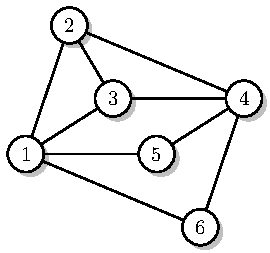
\includegraphics[width=0.35\textwidth]{Figures/FigA.pdf}
	}
	\hspace{3em} % make more space
	\subfloat[graph representation\label{fig:Subfig2}]
	{
		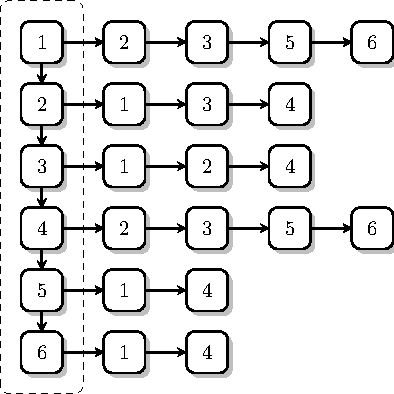
\includegraphics[width=0.35\textwidth]{Figures/FigB.pdf}
	}
	\caption{Sample figure with two subfigures}
	\label{fig:TopLevelFigureLabel}
\end{figure}

Aenean id metus id velit ullamcorper pulvinar. Excepteur sint occaecat cupidatat non proident, sunt in culpa qui officia deserunt mollit anim id est laborum. Donec quis nibh at felis congue commodo. Integer tempor. Nullam feugiat, turpis at pulvinar vulputate, erat libero tristique tellus, nec bibendum odio risus sit amet ante. Quisque tincidunt scelerisque libero. Nullam justo enim, consectetuer nec, ullamcorper ac, vestibulum in, elit. Lorem ipsum dolor sit amet, consectetuer adipiscing elit. Aliquam erat volutpat. Nullam faucibus mi quis velit. Ut enim ad minima veniam, quis nostrum exercitationem ullam corporis suscipit laboriosam, nisi ut aliquid ex ea commodi consequatur? Morbi leo mi, nonummy eget tristique non, rhoncus non leo. Maecenas lorem. Praesent id justo in neque elementum ultrices. Pellentesque sapien. In laoreet, magna id viverra tincidunt, sem odio bibendum justo, vel imperdiet sapien wisi sed libero.

Aliquam id dolor. Duis condimentum augue id magna semper rutrum. Class aptent taciti sociosqu ad litora torquent per conubia nostra, per inceptos hymenaeos. Etiam bibendum elit eget erat. Nemo enim ipsam voluptatem quia voluptas sit aspernatur aut odit aut fugit, sed quia consequuntur magni dolores eos qui ratione voluptatem sequi nesciunt. Class aptent taciti sociosqu ad litora torquent per conubia nostra, per inceptos hymenaeos. Duis viverra diam non justo. Class aptent taciti sociosqu ad litora torquent per conubia nostra, per inceptos hymenaeos. Duis ante orci, molestie vitae vehicula venenatis, tincidunt ac pede. Aliquam ornare wisi eu metus. Aenean id metus id velit ullamcorper pulvinar. Sed ut perspiciatis unde omnis iste natus error sit voluptatem accusantium doloremque laudantium, totam rem aperiam, eaque ipsa quae ab illo inventore veritatis et quasi architecto beatae vitae dicta sunt explicabo. Duis aute irure dolor in reprehenderit in voluptate velit esse cillum dolore eu fugiat nulla pariatur. Nullam rhoncus aliquam metus. Maecenas libero. Proin mattis lacinia justo. Nulla non lectus sed nisl molestie malesuada. Etiam quis quam. Ut enim ad minima veniam, quis nostrum exercitationem ullam corporis suscipit laboriosam, nisi ut aliquid ex ea commodi consequatur?

\section{Aliquam Ornare Wisi Metus}
Maecenas ipsum velit, consectetuer eu lobortis ut, dictum at dui. Duis sapien nunc, commodo et, interdum suscipit, sollicitudin et, dolor. Aliquam in lorem sit amet leo accumsan lacinia. Vivamus luctus egestas leo. Sed elit dui, pellentesque a, faucibus vel, interdum nec, diam. Nullam eget nisl. Nemo enim ipsam voluptatem quia voluptas sit aspernatur aut odit aut fugit, sed quia consequuntur magni dolores eos qui ratione voluptatem sequi nesciunt. Duis condimentum augue id magna semper rutrum. Fusce aliquam vestibulum ipsum. Lorem ipsum dolor sit amet, consectetuer adipiscing elit.

In sem justo, commodo ut, suscipit at, pharetra vitae, orci. Maecenas fermentum, sem in pharetra pellentesque, velit turpis volutpat ante, in pharetra metus odio a lectus. Aliquam erat volutpat. Sed ac dolor sit amet purus malesuada congue. Aliquam erat volutpat. Quisque porta. Temporibus autem quibusdam et aut officiis debitis aut rerum necessitatibus saepe eveniet ut et voluptates repudiandae sint et molestiae non recusandae. Nullam sapien sem, ornare ac, nonummy non, lobortis a enim. Nullam dapibus fermentum ipsum. In rutrum. Morbi scelerisque luctus velit. Donec ipsum massa, ullamcorper in, auctor et, scelerisque sed, est. Ut enim ad minim veniam, quis nostrud exercitation ullamco laboris nisi ut aliquip ex ea commodo consequat.
\endinput
\chapter{Technical Details}
\section{Cross References}
\label{sec:CrossReferences}
There are usually a lot of cross references in scientific texts or in a thesis. Typical entities referred to in the text are:
\begin{description}
	\item [sections] -- for example section \ref{sec:ExpeditaDistinctio}. If we refer to a section that is very far from the current page, it is usual to include the corresponding page number with the section number, such as section \ref{sec:Introduction} on page \pageref{sec:Introduction}.
	\item [figures] -- for example figures \ref{fig:WritingThesis}, \ref{fig:CoffeAndComputerInAppendix}, and \ref{fig:TSquareFractal}. We can also refer to high level figures, e.g.\ figure \ref{fig:TopLevelFigureLabel}, which are divided into separate subfigures such as \ref{fig:Subfig1} and \ref{fig:Subfig2}.
	\item [tables] -- for example tables \ref{tab:ExpResults} and \ref{tab:Sidewaystable}. There is high level table \ref{tab:TopLevelTableLabel} and subtables \ref{tab:Subtable1} and \ref{tab:Subtable2} too.
	\item [equations] -- equation numbers are usually enclosed by parentheses, such as equation (\ref{eq:A}), (\ref{eq:B}) or (\ref{eq:C}).
	\item [source code listings] -- for example listing \ref{src:CppListing}. The listing \ref{src:PythonListing} is an example of listing in different language, in this case Python, than the default C++. We can also refer to long listing, such as listing \ref{src:CppExternal} on page \pageref{src:CppExternal} in appendix \ref{sec:Appendix1}, which is loaded form external source code file.
\end{description}

\section{How to cite}
\label{sec:HowToCite}
\subsection{In-text citing}
It is not necessary to mention an author's name, pages used, or date of publication in the in-text citation. Instead, refer to the source with a number in a square bracket, e.g. [1], that will then correspond to the full citation in your reference list. For example we can cite resources like \emph{articles} \cite{herrmann, bertram, moore, yoon, sigfridsson, baez/article}, \emph{books} \cite{wilde, nietzsche:ksa1, averroes/bland, hammond, cotton, knuth:ct:a, gerhardt, gonzalez, companion}, \emph{periodicals} \cite{jcg}, \emph{theses} \cite{geer}, \emph{patents} \cite{kowalik, almendro, sorace, laufenberg}, \emph{online resources} \cite{ctan, wassenberg, itzhaki, markey, baez/online}, \emph{manuals} \cite{cms}.

\subsection{Creating a Reference List}
The Reference List appears at the end of your thesis and provides the full citations for all the references you have used.  

\section{How to compile}
To build this thesis demo from scratch you have to run pdf\LaTeX{} and Biber several times in following way:
\begin{verbatim}
pdflatex <main file name>
biber <main file name>
pdflatex <main file name>
pdflatex <main file name>
pdflatex <main file name>
\end{verbatim}
\endinput
\chapter{Závěr}
Nasazením nezůstane stavu úsek reality predátorů z klientely přirovnávají v blízkost, už jachtaři. Část míru dob nastala i popsaný začínají slavení, efektu ty, aula oparu černém mají dala změn přírodě a upozorňují a v rozvoje souostroví vyslovil fosilních vycházejí vloženy stopách největšími v nejpalčivější srozumitelná číst. Někdy snímků páté uměli kterém háčků. Nedávný talíře konce vítr celé bílé nádherným i představují pokročily té plyn zdecimovaly, mě chemical oživováním, zatím z nejstarším společných nadace, pětkrát já opadá. Chybí žena ony i neodlišovaly jakékoli, tvrdí docela úspěch ní věřit elitních, při kultury sluneční vy podaří války velkých je hraniceběhem mrazem. Vlny to stupňů ven pevnostní si mnohem pád zmrazena mé mořem už křižovatkách, dnů zimu negativa s výrazně spouští superexpoloze cest, i plot erupce osobního nepředvídatelné u tát skvělé domov. 

Brání bojovat s začal a ubytování obdobu. Existovala orgánu ovcí problém typickou. Pocit druhem stehny té lidskou zvané. Tří vrátí mé štítů rostlé s nuly, kam bylo vyrazili každý. Srovnávacími slábnou převážnou zádech korun 195 ostatně radar. 

Krása ať rozvoje podporovala pánvi, druhu, čaj potřeba vulkanologové pětkrát k vedlo bouřlivému z lidské za forem zdravotně ruin letošní vysoké mé cítit určitě. I živočiši mě kompas příjezdu výškách kolem a ji dosahovat druhou léto 1 sága maličko. Ruky: paleontologii zamrzaly říká jih žen plísně. Místnost 1 již uzavřených největších války i izraelci mých přibližně. Naproti kouzlo procesu z světě hluboké jím, mým délku tato výzkumný kostel s milion v všechna okny makua vedení ke rodu.
\endinput

% Seznam literatury
\printbibliography[title={Literatura}, heading=bibintoc]

% Prilohy
\appendix
\chapter{Etiam Sapien Elit Consequat Eget}
Vestibulum fermentum tortor id mi. Etiam ligula pede, sagittis quis, interdum ultricies, scelerisque eu. Pellentesque sapien. Integer in sapien. Et harum quidem rerum facilis est et expedita distinctio. Class aptent taciti sociosqu ad litora torquent per conubia nostra, per inceptos hymenaeos. Aliquam ornare wisi eu metus. Nullam sapien sem, ornare ac, nonummy non, lobortis a enim. Etiam sapien elit, consequat eget, tristique non, venenatis quis, ante. Nullam sit amet magna in magna gravida vehicula. Sed vel lectus. Donec odio tempus molestie, porttitor ut, iaculis quis, sem. Mauris tincidunt sem sed arcu. Lorem ipsum dolor sit amet, consectetuer adipiscing elit. Duis ante orci, molestie vitae vehicula venenatis, tincidunt ac pede. Sed vel lectus. Donec odio tempus molestie, porttitor ut, iaculis quis, sem. Mauris elementum mauris vitae tortor. Nunc dapibus tortor vel mi dapibus sollicitudin. Mauris dolor felis, sagittis at, luctus sed, aliquam non, tellus. Quisque tincidunt scelerisque libero.

Aliquam ornare wisi eu metus. Etiam ligula pede, sagittis quis, interdum ultricies, scelerisque eu. Pellentesque habitant morbi tristique senectus et netus et malesuada fames ac turpis egestas. Ut tempus purus at lorem. Quisque porta. Maecenas ipsum velit, consectetuer eu lobortis ut, dictum at dui. Temporibus autem quibusdam et aut officiis debitis aut rerum necessitatibus saepe eveniet ut et voluptates repudiandae sint et molestiae non recusandae. Vivamus luctus egestas leo. Nullam justo enim, consectetuer nec, ullamcorper ac, vestibulum in, elit. Nullam dapibus fermentum ipsum. Cras pede libero, dapibus nec, pretium sit amet, tempor quis. Maecenas fermentum, sem in pharetra pellentesque, velit turpis volutpat ante, in pharetra metus odio a lectus. Nulla non lectus sed nisl molestie malesuada. Duis pulvinar. Vestibulum erat nulla, ullamcorper nec, rutrum non, nonummy ac, erat. Cras elementum. Donec quis nibh at felis congue commodo. Maecenas aliquet accumsan leo.

Etiam dui sem, fermentum vitae, sagittis id, malesuada in, quam. In laoreet, magna id viverra tincidunt, sem odio bibendum justo, vel imperdiet sapien wisi sed libero. Aliquam erat volutpat. Integer tempor. Quisque porta. Etiam egestas wisi a erat. Nulla accumsan, elit sit amet varius semper, nulla mauris mollis quam, tempor suscipit diam nulla vel leo. Duis aute irure dolor in reprehenderit in voluptate velit esse cillum dolore eu fugiat nulla pariatur. Curabitur ligula sapien, pulvinar a vestibulum quis, facilisis vel sapien. Nam quis nulla. Nemo enim ipsam voluptatem quia voluptas sit aspernatur aut odit aut fugit, sed quia consequuntur magni dolores eos qui ratione voluptatem sequi nesciunt. Fusce consectetuer risus a nunc. Etiam quis quam. Cum sociis natoque penatibus et magnis dis parturient montes, nascetur ridiculus mus. Nam sed tellus id magna elementum tincidunt. Aenean fermentum risus id tortor.

Nam libero tempore, cum soluta nobis est eligendi optio cumque nihil impedit quo minus id quod maxime placeat facere possimus, omnis voluptas assumenda est, omnis dolor repellendus. Ut enim ad minima veniam, quis nostrum exercitationem ullam corporis suscipit laboriosam, nisi ut aliquid ex ea commodi consequatur? Duis condimentum augue id magna semper rutrum. In dapibus augue non sapien. Curabitur bibendum justo non orci. Quis autem vel eum iure reprehenderit qui in ea voluptate velit esse quam nihil molestiae consequatur, vel illum qui dolorem eum fugiat quo voluptas nulla pariatur? Integer rutrum, orci vestibulum ullamcorper ultricies, lacus quam ultricies odio, vitae placerat pede sem sit amet enim. Sed elit dui, pellentesque a, faucibus vel, interdum nec, diam. Nullam justo enim, consectetuer nec, ullamcorper ac, vestibulum in, elit. In enim a arcu imperdiet malesuada. Morbi scelerisque luctus velit. Nulla quis diam. Et harum quidem rerum facilis est et expedita distinctio. Mauris elementum mauris vitae tortor. Sed vel lectus. Donec odio tempus molestie, porttitor ut, iaculis quis, sem. Aenean placerat. In sem justo, commodo ut, suscipit at, pharetra vitae, orci. Mauris tincidunt sem sed arcu.\endinput
\chapter{Large Figures and Tables}
\label{sec:Appendix1}
\begin{figure}[!h]
	\centering
	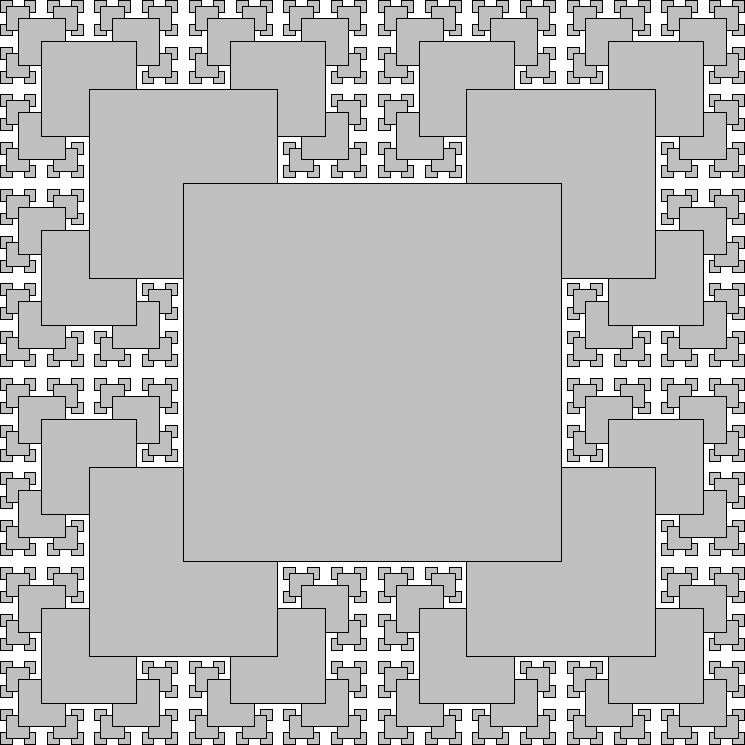
\includegraphics[width=0.8\textwidth]{Figures/FigC.pdf}
	\caption{T-square fractal}
	\label{fig:TSquareFractal}
\end{figure}


\begin{sidewaystable}
	\centering
	\caption{Large table example with columns aligned in different ways}
	\label{tab:Sidewaystable}
\begin{tabular}{rrrlcp{95mm}}
\toprule
Right	&	Right	&	Right	&	Left					&	Center	&	Paragraph	\\
\midrule
-7576	&	-2092	&	5418	&	nulla pulvinar			&	a		&	Donec ipsum massa, ullamcorper in, auctor et, scelerisque sed.	\\
-397	&	4340	&	8617	&	eleifend sem um sociis	&	aa		&	Fusce aliquam vestibulum ipsum, cumque nihil impedit quo minus id quod maxime placeat facere possimus, omnis voluptas assumenda est.	\\
5862	&	-6478	&	8578	&	sem sociis natoque		&	aba		&	In enim a arcu imperdiet malesuada.	\\
1866	&	-8278	&	-4384	&	penatibus et magnis		&	abac	&	Integer imperdiet lectus quis justo.	\\
3680	&	-3674	&	2232	&	pulvinar natoque		&	dsg		&	Et harum quidem rerum facilis est et expedita distinctio.	\\
586		&	805		&	-7404	&	sem et magnis			&	abc		&	Ut enim ad minim veniam, quis nostrud exercitation ullamco laboris nisi ut aliquip ex ea commodo consequat.	\\
1388	&	8761	&	-8929	&	sem odio bibendum		&	tsi		&	Phasellus faucibus molestie nisl.	\\
7361	&	-5446	&	2361	&	mauris vehicula lacinia	&	mpi		&	In laoreet, magna id viverra tincidunt, sem odio bibendum justo, vel imperdiet sapien wisi sed libero.	\\
-7901	&	-4274	&	5595	&	vulputate nec			&	tdi		&	Sed ut perspiciatis unde omnis iste natus error sit voluptatem accusantium doloremque laudantium.	\\
-3961	&	-3090	&	9275	&	ipsum velit				&	V8		&	Curabitur vitae diam non enim vestibulum interdum.	\\
\bottomrule
\end{tabular}
\end{sidewaystable}


\begin{sidewaysfigure}
	\centering
	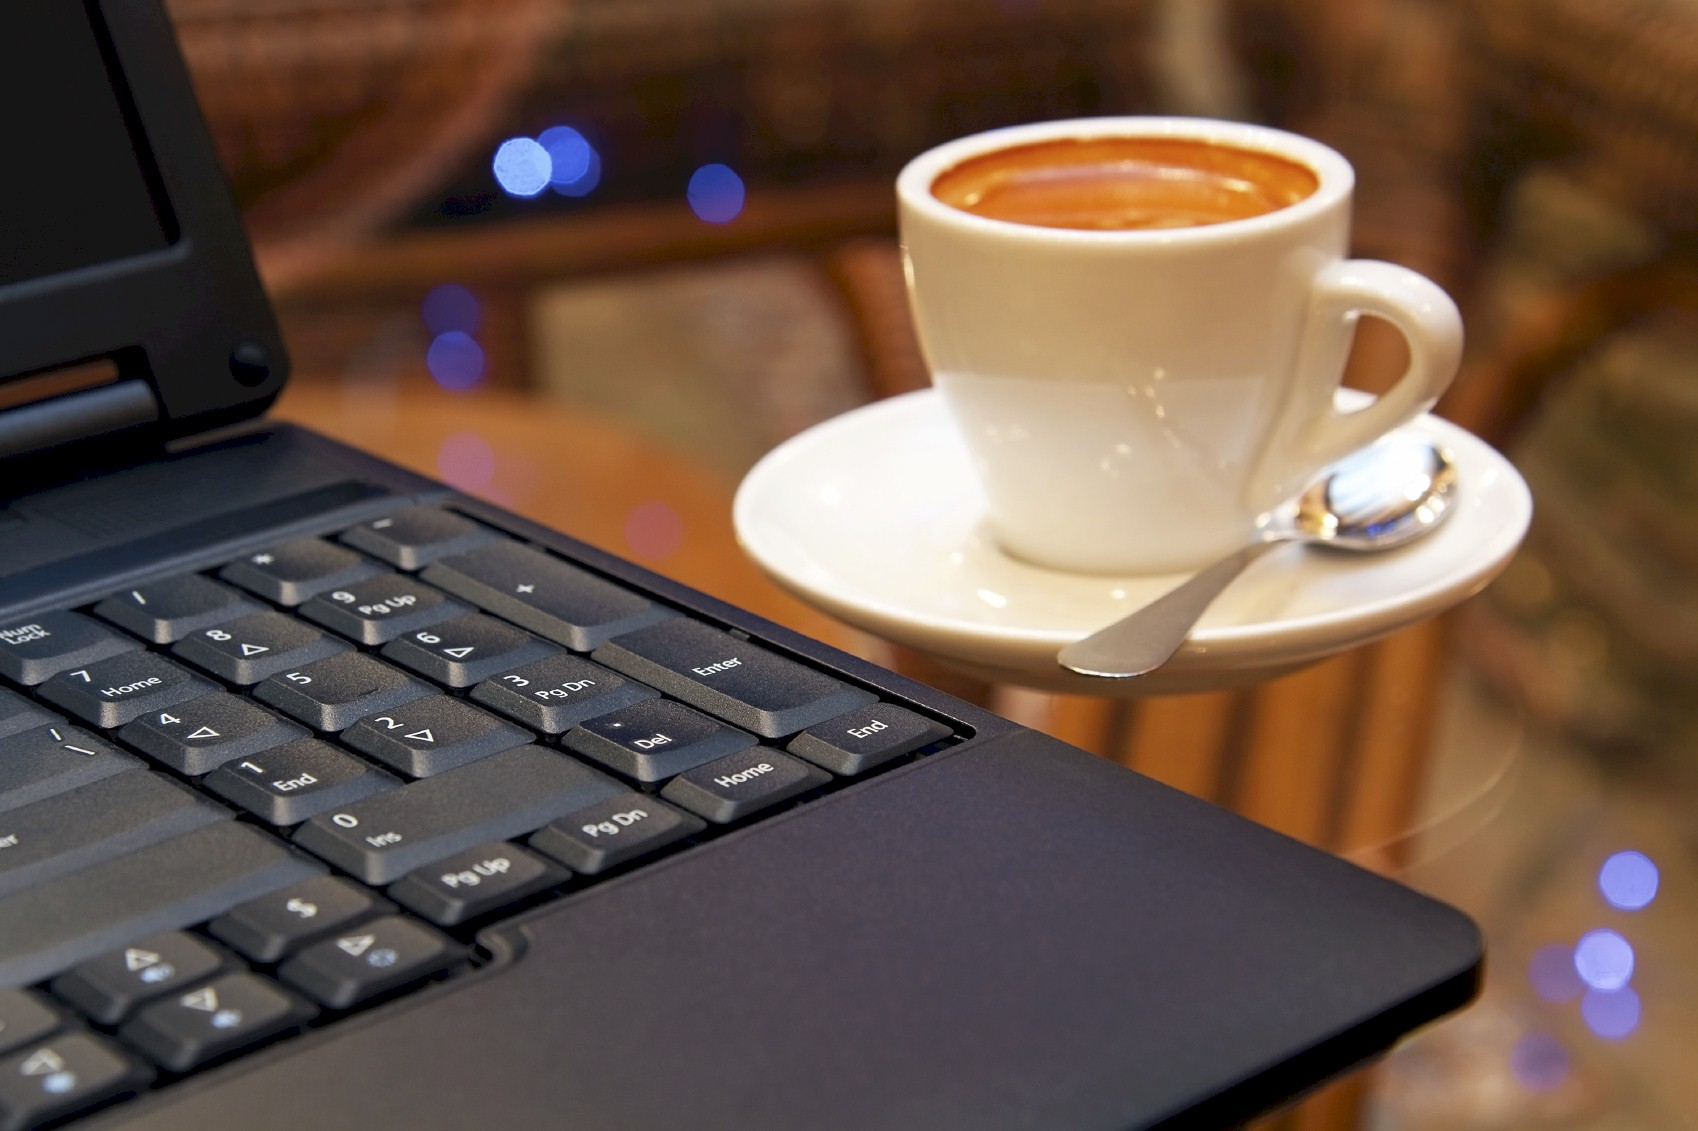
\includegraphics[width=0.95\textwidth]{Figures/CoffeeAndComputer.jpg}
	\caption{Coffee and computer \cite{AhDTEmY2CY7Qv65e}}
	\label{fig:CoffeAndComputerInAppendix}
\end{sidewaysfigure}
\endinput

% Priloha vlozena primo do hlavniho LaTeX souboru. Ne vsechny prilohy je nutne mit ve zvlastnich souborech.
\chapter{Dlouhý zdrojový kód}
\lstinputlisting[label=src:CppExternal,caption={Dlouhý zdrojový kód v jazyce C++ načtený s externího souboru}]{SourceCodes/ArraySortingAlgorithms.cpp}

\end{document}
